\section{Introduction}
\label{sec:introduction}
Strong gravitational lensing by intervening galaxies splits a gravitational-wave (GW) signal into several images that arrive with relative delays of minutes to months, with different magnifications and with discrete Morse phase shifts \citep{takahashi2003waveeffects,dai2017morse,ezquiaga2021phase}. Current detectors are expected to observe roughly one strongly lensed binary-black-hole (BBH) pair per thousand detections, rising to hundreds of pairs per year for third-generation instruments such as the Einstein Telescope \citep[ET;][]{ng2018rates,li2018statistical,oguri2018distribution,wierda2021beyond}. Searches of the LIGO--Virgo--KAGRA (LVK) data through the fourth observing run have not yet produced a confident multiple-image detection \citep{hannuksela2019search,lvk2021o3a,lvk2024o3search,lvk2025gwtc4lensing}, but the rapidly growing catalog \citep{lvk2025gwtc4} makes the first detections a realistic near-term prospect.

A lensed GW image has strain amplitude proportional to $\sqrt{|\mu|}/d_L$, where $\mu$ is its signed magnification and $d_L$ the luminosity distance of the source. GW data alone therefore measure only the apparent distance $d_L/\sqrt{|\mu|}$ of each image and the \emph{relative} magnifications between images. Correcting the luminosity distance---for cosmography, tests of GW propagation or population studies \citep{liao2017precision,oguri2019review}---requires the \emph{absolute} magnification of at least one image. This in turn requires a lens model, which must be constrained by electromagnetic (EM) observations of the lens and of the lensed host galaxy \citep{hannuksela2020localizing,wempe2022lensing,smith2023discovering,uronen2026galacticcentres}. The mass-sheet degeneracy \citep{falco1985msd,schneider2013msd} implies that image positions and flux ratios alone cannot fix the absolute magnification: an assumption about, or an independent measurement of, the radial mass profile and the external convergence is required.

Combining GW relative magnifications and time delays with an EM reconstruction of the lens to obtain absolute magnifications and source distances is not new. \citet{hannuksela2020localizing} demonstrated the principle, including the distance reconstruction, for representative systems. \citet{wempe2022lensing} studied the joint GW and EM selection and host localization of lensed BBHs. \citet{poon2025degeneracy} derived which lens and source quantities GW lensing can identify and how the mass-sheet and similarity degeneracies enter. \citet{uronen2026silmarel} built a joint Bayesian reconstruction framework that adds Gaussian likelihood terms for the GW relative magnifications and delays to an EM lens model, and \citet{uronen2026galacticcentres} applied this approach to locating BBHs within their hosts. What has not been established is how accurate and how \emph{reliable} absolute-magnification estimates are across realistic lens and source populations: when the quoted uncertainty can be trusted, when it is set by the prior rather than the data, and when it fails. Magnification benchmarks of this kind exist for cluster lenses \citep{meneghetti2017ff}, but not for galaxy-scale lensed GWs.

This paper provides such a benchmark. We address five questions. (i) How much information do image geometry, the GW magnification ratio and arrival order, the GW delay and SNRs, and spectroscopic follow-up each contribute, and which of them make the estimate depend on an assumed distance--redshift relation? (ii) How does accuracy degrade near caustics? (iii) Do the quoted 90\% intervals contain the true value 90\% of the time (i.e. are they calibrated), for each lens family, when the family is unknown, and when the assumed lens model is wrong? (iv) Is our simplified, SNR-based model of the GW measurements adequate, judged against full Bayesian parameter estimation of both images from simulated detector data? (v) How do estimators trained on simulations compare with a conventional Bayesian lens reconstruction that uses the same observables and priors? Our benchmark (a) draws BBH sources from the GWTC-4.0 population model \citep{lvk2025gwtc4pop} with optical-depth weighting, (b) uses four galaxy-lens families with observationally motivated shape distributions, (c) applies the same detection criterion and the same requirement that the images be resolved to all families for an O5-like network and for ET, (d) calibrates the GW distance errors on the 167 BBH events of GWTC-1 to GWTC-4.0, tests the relative-amplitude error model by injections into public O4a strain and by joint parameter estimation of lensed image pairs, and (e) compares two estimators trained on the simulations---gradient-boosted decision trees and neural posterior estimation---with conventional Bayesian posteriors on a representative subset.

Section~\ref{sec:physics} summarizes the lens physics and the mass-sheet degeneracy. Section~\ref{sec:simulation} describes the simulations and the observation model, and Sec.~\ref{sec:realdata} its calibration and validation on real data. Section~\ref{sec:inference} describes the inference methods, Sec.~\ref{sec:results} presents the benchmark results, Sec.~\ref{sec:pe} the parameter-estimation and Bayesian reconstruction tests, and Sec.~\ref{sec:discussion} discusses their implications and limitations.

\section{Lensing of gravitational waves}
\label{sec:physics}
\subsection{Geometric-optics images}
In the thin-lens approximation, the lensed frequency-domain waveform is $\tilde h_L(f)=F(f)\tilde h(f)$. For the galaxy-scale lenses considered here $f\,\Delta t\gg1$ in the detector band and geometric optics applies,
\begin{equation}
F(f)=\sum_j |\mu_j|^{1/2}\exp\left(2\pi i f t_j-i\pi n_j\right),
\label{eq:go}
\end{equation}
where $t_j$ is the arrival time of image $j$ and $n_j=0,\tfrac12,1$ for minima, saddle points and maxima of the Fermat potential \citep{schneider1992gravitationallenses,takahashi2003waveeffects,dai2017morse}. The signed magnification is the inverse determinant of the lens-mapping Jacobian $A=\partial\boldsymbol\beta/\partial\boldsymbol\theta$,
\begin{equation}
\mu=\left(\det A\right)^{-1}=\left[(1-\kappa)^2-|\gamma|^2\right]^{-1},
\label{eq:jacobian}
\end{equation}
with convergence $\kappa$ and shear $\gamma$. The sign of $\mu$ gives the image parity. In the rest of the paper $\mu_A$, $\mu_B$ and the magnification ratio $\mu_B/\mu_A$ denote absolute values $|\mu|$; the image type is carried separately by the Morse index. Near a fold caustic $\det A\to0$, so a perturbation $\delta A$ changes the magnification by $\delta\ln|\mu|=-\operatorname{tr}(A^{-1}\delta A)$, which diverges as $|\mu|$; small errors in the reconstructed lens or source position therefore produce large magnification errors for highly magnified images.

For a singular isothermal sphere (SIS) with Einstein radius $\theta_E$ and dimensionless source offset $y=\beta/\theta_E<1$, the two images lie at $\theta_\pm=\theta_E(1\pm y)$ on opposite sides of the lens with
\begin{equation}
\begin{gathered}
\mu_\pm=1\pm\frac1y,\qquad \frac{|\mu_-|}{\mu_+}=\frac{1-y}{1+y},\\
\Delta t=\frac{(1+z_l)}{c}\frac{D_lD_s}{D_{ls}}\,2y\,\theta_E^2 .
\end{gathered}
\label{eq:sis}
\end{equation}
Here $D_l$, $D_s$ and $D_{ls}$ are angular-diameter distances. In general the delay between two images is $\Delta t=D_{\Delta t}\Delta\phi/c$, with the time-delay distance $D_{\Delta t}\equiv(1+z_l)D_lD_s/D_{ls}$ and the Fermat-potential difference $\Delta\phi$ in angular units (rad$^2$); for the SIS, $\Delta\phi=2y\theta_E^2$. The image-position asymmetry $(\theta_+-\theta_-)/(\theta_++\theta_-)=y$ and the flux ratio each determine $y$ and therefore $\mu_\pm$ within the SIS model; the inversion becomes unstable as $y\to0$ because $d\mu_+/dy=-y^{-2}$.

\subsection{Mass-sheet degeneracy and the distance scale}
\label{sec:msd}
The transformation $\kappa\to\lambda\kappa+(1-\lambda)$, $\boldsymbol\beta\to\lambda\boldsymbol\beta$ leaves image positions and magnification ratios invariant, rescales all magnifications as $\mu\to\mu/\lambda^2$ and, at fixed time-delay distance, the delays as $\Delta t\to\lambda\Delta t$ \citep{falco1985msd,schneider2013msd}. An external convergence $\kappa_{\rm ext}$ acts in this way with $\lambda=1-\kappa_{\rm ext}$. It is only one realization of the degeneracy: an internal mass sheet, or more generally a change of the radial profile of the lens galaxy (e.g. its power-law slope), changes the magnification at fixed image configuration as well \citep{schneider2013msd}. Setting $\kappa_{\rm ext}=0$ therefore does not make the magnification independent of the assumed mass profile, and all our results are conditional on the simulated lens populations, including their slope distribution. Image geometry, the GW relative magnification and the arrival order are therefore blind to $\lambda$. A double-image system has only one delay, so it provides no dimensionless delay ratio, and its dimensional delay is \emph{not} invariant. The degeneracy can be broken by an absolute GW amplitude combined with a known source redshift and an assumed cosmology, by the measured delay combined with an independent time-delay distance \citep{poon2025degeneracy}, or by stellar kinematics interpreted with a dynamical model. The first two require an assumed distance--redshift relation; kinematics constrain the mass through distance ratios but depend on the dynamical modeling and constrain only the internal part of the mass sheet.

These relations define the cosmology dependence of an estimator. Let $f$ use only invariant inputs. For a fixed system and image identification, $f(\boldsymbol x_\lambda)=f(\boldsymbol x)$, so its estimate relative to the transformed truth is $\hat\mu_\lambda/\mu_\lambda=\lambda^2\,\hat\mu/\mu$: the mass sheet multiplies the estimator's own error by $\lambda^2$. The same inputs contain no distance scale, so $f$ is unaffected by the assumed cosmology except through the population prior (for example through the lens-redshift and velocity-dispersion distributions). An estimator that also uses the delay, the SNRs or an apparent distance together with redshifts can learn the simulated distance--redshift relation from the simulated events on which it is trained (its training set). It then depends on the assumed cosmology, and its response to $\lambda$ must be measured rather than derived. All simulations below have $\lambda=1$; Secs.~\ref{sec:information} and \ref{sec:pe} test the response to $\lambda\neq1$ and to a different distance scale.

\section{Simulations}
\label{sec:simulation}
We generate catalogs of independent lens systems for four lens families, evaluating each system for two detector scenarios. Table~\ref{tab:simulation} summarizes the ingredients.

\begin{table*}
\centering\papertablestyle
\caption{Simulation ingredients. All lens systems are independent: no source or lens parameters are reused between events.}
\label{tab:simulation}
\begin{tabularx}{\linewidth}{@{}p{.18\linewidth}L@{}}
\toprule
Component & Model \\
\midrule
BBH masses & GWTC-4.0 \textsc{Broken Power Law + 2 Peaks}, posterior medians \citep{lvk2025gwtc4pop}: $\alpha_1=1.7$, $\alpha_2=4.5$, $m_{\rm break}=36\,{\rm M_\odot}$, peaks at $9.8$ and $33\,{\rm M_\odot}$ \\
Spins & aligned components of the GWTC-4.0 default spin model \\
Source redshift & $p(z_s)\propto \psi(z_s)(1+z_s)^{-1}\,{\rm d}V_c/{\rm d}z_s\,\tau(z_s)$; $\psi$ Madau--Dickinson shape \citep{madau2014cosmic} with low-$z$ slope 3.2; $\tau\propto D_C^3(z_s)$; $0.1<z_s<10$ \\
Lens redshift & $p(z_l|z_s)\propto (D_{C,l}D_{C,ls}/D_{C,s})^2$ \citep{turner1984statistics} \\
Velocity dispersion & SDSS early-type velocity-dispersion function \citep{choi2007vdf} weighted by $\sigma_v^4$, $100<\sigma_v<400\,{\rm km\,s^{-1}}$ \\
Lens families & SIS; SIE with $q\sim\mathcal N(0.75,0.15)$ on $[0.35,0.99]$ \citep{bolton2008slacs}; SIE + external shear, $|\gamma_{\rm ext}|$ log-normal with median 0.05; elliptical power law (EPL) + shear with slope $\gamma'\sim\mathcal N(2.08,0.15)$ \citep{auger2010slacs,tessore2015epl} \\
Source position & uniform in area within $(1.0$--$1.8)\,\theta_E$, redrawn until multiply imaged; the cross-section weighting enters through $\sigma_v^4$ only, not through the lens shape \\
Images & lenstronomy \citep{birrer2018lenstronomy,birrer2021lenstronomy} root finding with residual check; signed $\mu$, $\kappa$, Morse index and Fermat delay per image \\
Detector networks & O5-like: H1, L1 at A+ and V1 at AdV design, $f_{\min}=10$\,Hz; ET-D triangle \citep{hild2011etd}, $f_{\min}=5$\,Hz; IMRPhenomXAS \citep{pratten2020xas}; antenna patterns at each image's arrival time \\
Detection & matched-filter network SNR $\hat\rho_j=\rho_j+\mathcal N(0,1)\ge8$ for two images arriving within one year; pair separation $\ge0.1$\,arcsec \\
GW measurements & relative magnification, apparent distances, delay; errors from SNR, sky/orientation uncertainty and GWTC-calibrated inclination term (Sec.~\ref{sec:gwmeas}) \\
EM measurements & image positions $\pm0.01$\,arcsec; lens-light center $\pm0.02$\,arcsec; light axis ratio $\pm0.05$; light--mass misalignment $10^\circ$; spectroscopic $z_l,z_s$ ($\sigma_z=10^{-3}(1+z)$); $\sigma_v$ to 10\% \\
Frame & random true lens center ($\mathcal N(0,5\,{\rm arcsec})$ per axis) and random rotation \\
\bottomrule
\end{tabularx}
\end{table*}

\subsection{Sources and lenses}
Source masses and spins follow the fiducial GWTC-4.0 BBH population, whose population parameters we take directly from the machine-readable summary of \citet{lvk2025gwtc4pop}. Source redshifts follow the merger-rate density, the comoving volume and the strong-lensing optical depth of a non-evolving isothermal lens population, $\tau\propto D_C^3(z_s)$ \citep{turner1984statistics}; the resulting lensed-source redshift distribution peaks near $z_s\approx3$. For each source, a lens redshift is drawn from the isothermal lensing kernel and a velocity dispersion from the SDSS velocity-dispersion function weighted by the isothermal cross-section $\propto\sigma_v^4$ \citep{choi2007vdf,haris2018identifying}. The Einstein radius follows from the SIS relation in the Planck18 cosmology \citep{planck2020cosmology}. For the elliptical families the same normalization is used. The source is drawn uniformly in area within a disk of radius $1.6$--$1.8\,\theta_E$ ($\theta_E$ for the SIS) and redrawn until the lens produces at least two images, so it is uniform over the multiple-image region of each lens, the set of source positions that produce at least two images. Quadruple-image systems therefore occur at their natural rate for each lens, but lenses are not weighted by the dependence of the area of that region on their shape and slope.

\subsection{GW measurements}
\label{sec:gwmeas}
For each source we compute the face-on noise-weighted inner products $I_{0,d}=4\int|\tilde h_0|^2/S_d\,{\rm d}f$ for every detector $d$, so that the optimal SNR of image $j$ is
\begin{equation}
\rho_j^2=|\mu_j|\sum_d I_{0,d}\left[F_{+,d}^2\left(\frac{1+\cos^2\iota}{2}\right)^2+F_{\times,d}^2\cos^2\iota\right]_{t=t_j},
\end{equation}
with antenna patterns evaluated at the arrival time of each image. Because the Earth rotates between images, the antenna response differs between images by factors of up to several, so flux ratios cannot be read directly from SNR ratios. The relative magnification is estimated as
\begin{equation}
\ln\widehat{\left(\frac{\mu_B}{\mu_A}\right)}=2\ln\frac{\hat\rho_B}{\hat\rho_A}-2\ln\frac{\hat R_B}{\hat R_A},
\end{equation}
where $\hat R_j$ is the network response evaluated at an estimated sky position, polarization and inclination. These are shared by both images in a joint analysis \citep{janquart2023golum,lo2023bayesian}; we perturb them with errors that scale as $20/\rho_{\rm joint}$ times $2^\circ$ (O5) or $15^\circ$ (ET alone) on the sky, 0.5\,rad in polarization and 0.3 in $\cos\iota$. We also store the optimistic known-sky estimate. The apparent distance of each image, $D_{{\rm app},j}=d_L/\sqrt{|\mu_j|}$, is measured with the same SNR and response errors plus a shared inclination--distance term calibrated on real events (Sec.~\ref{sec:realdata}).

\subsection{EM observations and selection}
At the data level, the GW observations are strain time series containing the separate lensed arrivals, and the EM observations are high-resolution images of the lens and the lensed host together with spectra. The benchmark operates on simulated summaries of these data. We assume that the host has been identified and that the image positions of the BBH within the lensed host have been reconstructed \citep{hannuksela2020localizing,wempe2022lensing,uronen2026galacticcentres}. This is an upstream inference, not a direct observation: the BBH is not seen in the EM data, and its image positions follow from a model of the extended host together with the GW information. All results are therefore conditional on the stated astrometric precision of the GW-source images, and Sec.~\ref{sec:pe} tests how they degrade when it is worse. Image positions carry 0.01\,arcsec errors and the lens-light center 0.02\,arcsec; the lens light traces the mass axis ratio and orientation with scatter. Spectroscopic redshifts of the lens and host and the lens velocity dispersion are available as follow-up. The velocity dispersion is used only as a measure of the lens strength: it is the SIS-equivalent $\sigma_v$ that sets the Einstein radius in the simulation, observed with 10\% scatter, not a stellar-kinematic observable interpreted with a dynamical model. It is unaffected by an external convergence but would change under an internal mass-sheet transformation. The true lens center and the frame orientation are random, and all inputs are invariant under translations and rotations of the image (Sec.~\ref{sec:features}). A system is selected for a scenario if two images have $\hat\rho\ge8$ within one year and the GW image pair is separated by at least 0.1\,arcsec, comparable to the resolution of space-based imaging.

\section{Real-data calibration and validation}
\label{sec:realdata}
\subsection{Distance uncertainties from GWTC-1 to GWTC-4.0}
We queried the GWOSC event service \citep{gwosc2023} for all confident BBH candidates in GWTC-1, GWTC-2.1, GWTC-3 and GWTC-4.0 (167 events with published distance credible intervals). Converting the 90\% intervals into log-normal widths, the uncertainty is well described by
\begin{equation}
\sigma_{\ln d_L}(\rho)=\sqrt{a^2+(b/\rho)^2},
\end{equation}
with $a=0.223\pm0.013$, $b=2.74\pm0.12$ and an rms residual of 0.057 (Fig.~\ref{fig:realdata}a). The constant term reflects the inclination--distance degeneracy, which does not average down with SNR \citep{cutler1994gravitational}; $b>1$ shows that the amplitude uncertainty at finite SNR is inflated by parameter correlations. In the simulation we split the single-image error into the explicit SNR and response terms and a shared term with variance $a^2+(b^2-1)/\rho_{\rm joint}^2$, so that a single image reproduces the catalog uncertainties while the relative magnification---for which inclination is common to both images---is limited by SNR and antenna-pattern errors.

\subsection{Relative amplitudes in O4a detector noise}
The relative-magnification error model assumes Gaussian, stationary noise. We tested it by injecting lensed image pairs into public O4a strain from LIGO Hanford and Livingston \citep{gwosc2023}. Ten 4096-s frame files (five H1/L1 blocks) were used; analysis segments of 64\,s with good data-quality flags were whitened with a median-Welch PSD estimated from the preceding 512\,s. Each pair consists of the same IMRPhenomXAS source injected with magnifications $\mu_A$ and $\mu_B$ into two independent segments, at network SNR between 10 and 60 for the brighter image. Each image was recovered by matched filtering with the exact template, maximized over phase and a $\pm5$\,ms window. The same injections were repeated in colored Gaussian noise with identical PSDs as a control.

Fig.~\ref{fig:realdata}(b) shows the standardized error $z=[\ln(\hat\mu_B/\hat\mu_A)-\ln(\mu_B/\mu_A)]/\sigma_{\rm model}$ with $\sigma_{\rm model}=2(\rho_A^{-2}+\rho_B^{-2})^{1/2}$ for the 321 pairs with both images above $\rho=8$. In Gaussian noise the standard deviation of $z$ is 0.94 (Kolmogorov--Smirnov $p=0.15$ against a unit normal). In O4a noise the robust (median-absolute-deviation) standard deviation is 1.02 and the median absolute error of $\ln(\mu_B/\mu_A)$ is 0.074, against 0.067 in Gaussian noise. A single pair (0.3\%) is a catastrophic outlier: a loud glitch within the timing window raises the recovered SNR of the fainter image from 27 to 213. Excluding it, the standard deviation is 1.01. The Gaussian amplitude-error model therefore describes real O4a noise well, provided glitch-contaminated images are removed by standard signal-consistency vetoes or glitch subtraction.

\begin{figure*}
\centering
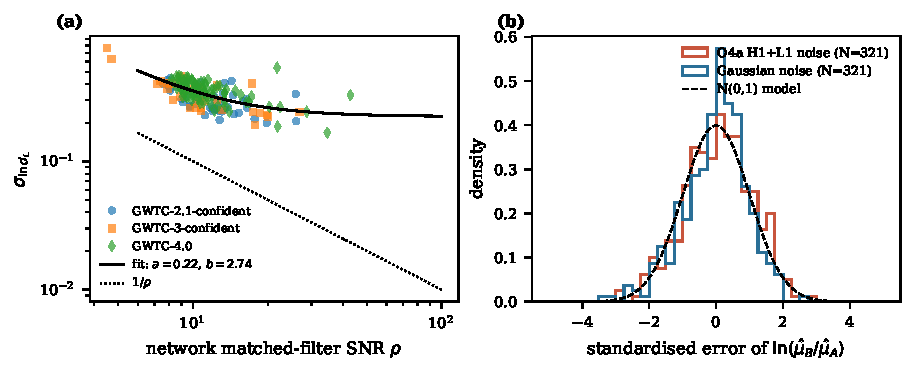
\includegraphics[width=\linewidth]{fig_realdata.pdf}
\caption{Real-data calibration and validation. (a) Log-distance uncertainty versus network matched-filter SNR for 167 confident BBH events in GWTC-1 to GWTC-4.0, with the fitted model used in the simulations. (b) Standardized error of the recovered relative magnification for lensed image pairs injected into public O4a H1/L1 strain and into Gaussian noise with the same PSDs. One glitch-contaminated O4a pair ($z=44.5$) lies outside the plotted range.}
\label{fig:realdata}
\end{figure*}

\section{Inference}
\label{sec:inference}
\subsection{Observables}
\label{sec:features}
The target is the absolute magnification $\mu_A$ of the GW image with the larger measured network SNR (image $A$). The image-geometry observables are the radii of images $A$ and $B$ from the observed lens-light center, their separation, opening angle and asymmetry, an Einstein-radius proxy $(r_A+r_B)/2$, the number of resolved images and the normalized radii of any additional images, the light axis ratio, and the image position angles relative to the light major axis. The GW observables are the magnification ratio $\ln(\hat\mu_B/\hat\mu_A)$ and the arrival order ${\rm sign}(\Delta t)$, which together we call the ``$\mu$ ratio'' below; the delay $\ln|\Delta t|$, which carries a time scale; the two SNRs, which are dimensionless but carry the absolute amplitude and hence depend on the source distance; and the two apparent distances. The follow-up observables are the spectroscopic redshifts $z_l$, $z_s$ and $\ln\sigma_v$. Finally, the estimate $\ln\hat\mu_{\rm cosmo}=2[\ln d_L(\hat z_s)-\ln\hat D_{{\rm app},A}]$ uses the measured source redshift with the Planck18 distance--redshift relation.

Table~\ref{tab:inputsets} lists the combinations of observables that we compare; each is named after the observables it contains. Three properties must be distinguished. The image geometry and the $\mu$ ratio are invariant under the mass-sheet transformation of Sec.~\ref{sec:msd}, and the redshifts and $\sigma_v$, a property of the lens galaxy, are unchanged by an external convergence. None of these observables contains a time or distance scale, so an estimator that uses only them cannot learn the distance--redshift relation of the simulations. We call the four combinations built from them scale-free. Adding the delay and the SNRs introduces a time and an amplitude scale. Without redshifts this adds little (Sec.~\ref{sec:information}); with redshifts, an estimator trained on simulations in one cosmology can relate the delay to the time-delay distance and the SNRs to the luminosity distance, so its output depends on that cosmology even though no distance--redshift relation is supplied explicitly. ``GW\,+\,$z$'' and ``All observables'' contain $\hat\mu_{\rm cosmo}$ explicitly. Distance corrections from these four combinations are therefore circular for cosmography.

\begin{table}
\centering\papertablestyle
\caption{Combinations of observables. ``Scale-free'' combinations are invariant under an external mass sheet and contain no time or distance scale. ``$\mu$ ratio'': the GW magnification ratio $\ln(\hat\mu_B/\hat\mu_A)$ and the arrival order ${\rm sign}(\Delta t)$.}
\label{tab:inputsets}
\begin{tabularx}{\columnwidth}{@{}lLc@{}}
\toprule
Name & Observables & Scale-free \\
\midrule
GW only & $\mu$ ratio, $\ln|\Delta t|$, SNRs, apparent distances & no \\
GW\,+\,$z$ & GW only + $z_l$, $z_s$, $\sigma_v$ + $\hat\mu_{\rm cosmo}$ & no \\
Geometry & image geometry relative to the lens-light center, light shape & yes \\
Geometry\,+\,$z,\sigma_v$ & Geometry + $z_l$, $z_s$, $\sigma_v$ & yes \\
Geometry\,+\,$\mu$ ratio & Geometry + $\ln(\hat\mu_B/\hat\mu_A)$, ${\rm sign}(\Delta t)$ & yes \\
Geometry\,+\,$\mu$ ratio\,+\,$z,\sigma_v$ & the above + $z_l$, $z_s$, $\sigma_v$ & yes \\
Geometry\,+\,$\mu$ ratio\,+\,$\Delta t$, SNR & Geometry\,+\,$\mu$ ratio + $\ln|\Delta t|$, SNRs & no \\
Geometry\,+\,$\mu$ ratio\,+\,$\Delta t$, SNR\,+\,$z,\sigma_v$ & the above + $z_l$, $z_s$, $\sigma_v$ & no \\
All observables & all of the above + apparent distances, $\hat\mu_{\rm cosmo}$ & no \\
\bottomrule
\end{tabularx}
\end{table}

\subsection{Estimators and their uncertainties}
We use two estimators that are constructed (trained) from simulated events. The first is gradient-boosted decision trees in the histogram-based implementation of \textsc{scikit-learn} \citep[hereafter HistGB;][]{pedregosa2011scikit}, trained to predict directly the 5th, 50th and 95th percentiles of $\ln\mu_A$ given the inputs (quantile regression). These percentile estimates need not contain the truth 90\% of the time, so we calibrate them with conformalized quantile regression \citep[CQR;][]{romano2019cqr}. On a separate set of simulated events (the calibration set) we compute for each event how far the true value $y_i$ lies outside its predicted interval, $s_i=\max(\hat q_{05,i}-y_i,\,y_i-\hat q_{95,i})$ (negative if inside), and then widen or narrow all intervals by the value of $s$ that 90\% of the calibration events do not exceed (the $\lceil(n+1)0.9\rceil$-th smallest of the $n$ values). This guarantees 90\% coverage on average over events drawn from the same population as the calibration set, without assuming a Gaussian error distribution. The correction is computed either once for all events (global calibration) or separately within groups of events \citep{vovk2005algorithmic}. The groups are defined either by observed quantities---the number of resolved images or bins of the predicted magnification---or by the true lens family. The latter is a diagnostic only, because the family of a real lens is not known; as an alternative that does not need it, we also calibrate every event on the EPL+shear calibration events alone. Coverage estimates are quoted with binomial uncertainties where they are compared with the nominal level. All simulated events are independent. For each family they are divided at random into 60\% for training, 20\% for calibration and 20\% for testing, on which all results are quoted, and we repeat this with five different random divisions (three for experiments that mix families). Up to 60\,000 selected events per family and scenario are used.

The second estimator is neural posterior estimation \citep[NPE;][]{papamakarios2016fast}, the simulation-based method that has also been used for rapid GW parameter estimation \citep{dax2021neuralposterior}. A neural network---a conditional normalizing flow with spline transformations \citep{durkan2019nsf}, implemented in \textsc{zuko} \citep{rozet2022zuko}---is trained on simulated events to represent the posterior density $p(\ln\mu_A\,|\,\boldsymbol x)$ of the magnification given the inputs $\boldsymbol x$. The posterior median provides the point estimate. We check calibration with the coverage of central intervals at several levels and with the probability integral transform (PIT), the posterior probability below the true value, which is uniformly distributed over events when the posteriors are calibrated.

As a reference without event information we use a prior-only predictor that ignores the event data and returns the percentiles of $\ln\mu_A$ in the training events of the same family. We also evaluate three closed-form estimators: the SIS asymmetry inversion (Eq.~(\ref{eq:sis})), the SIS inversion of the measured relative magnification, and $\hat\mu_{\rm cosmo}$. We report the median relative error $|\hat\mu-\mu|/\mu$, the mean absolute error (MAE) of $\mu_A$, the fraction of events with relative error below 10\%, and the interval coverage (the fraction of events whose true value lies inside the interval) and mean log-width.
